\section{Parallelisierung der kritischen Abschnitte}

\subsection{Parallelisierung}
\begin{frame}{Parallele Verarbeitung einzelner Bildpaare}
	\centering
	\begin{tikzpicture}
		\node at (-5,0) {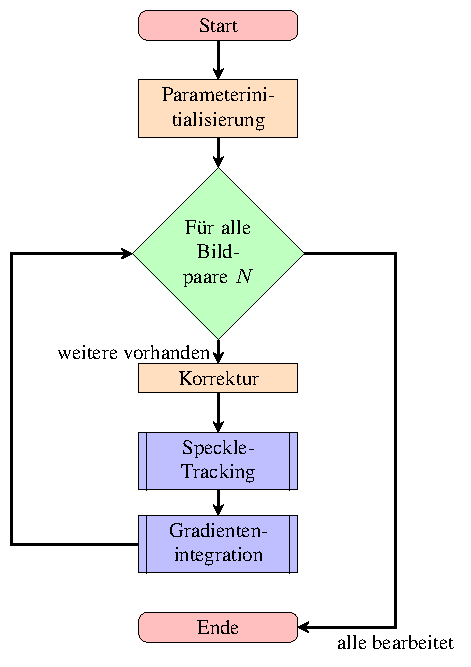
\includegraphics[width=0.4\linewidth]{pdf/graph_main}};
		
		\draw[blue, very thick] (-6.2, -0.0) rectangle (-4.1, -2.6);
		
		\node at (-1,0) {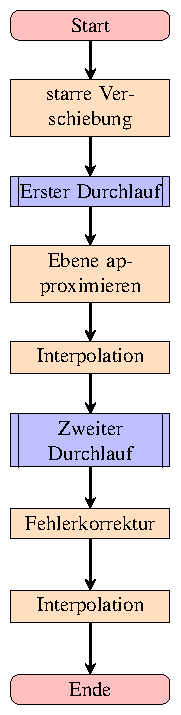
\includegraphics[width=0.16\linewidth]{pdf/graph_speckle}};
		
		\draw[red!50, very thick] (-6, -1.6) rectangle (-4.3, -0.85);
		\draw[red!50, very thick] (-4.3, -0.85) -- (-2, 3.7);
		\draw[red!50, very thick] (-4.3, -1.6) -- (-2, -3.7);
		\draw[red!50, very thick] (-2, -3.7) rectangle (0.1, 3.7);
		
		\draw[green, very thick] (-1.9, -1.2) rectangle (-0.1, -0.5);
		
		\node[draw=green] at (2, 1) {multiprocessing};
		\node[draw=blue] at (2, 0) {MPI};
	\end{tikzpicture}
\end{frame}

\begin{frame}{Parallele Verarbeitung einzelner Bildpaare}
	\textbf{Benennung:} \textit{mpi}
	\begin{enumerate}
		\item Verteilung einzelner Bildpaare auf Rechenkerne
		\item parallele Verarbeitung mittels MPI und multiprocessing
		\item Sammeln der Daten auf dem Masterkern
	\end{enumerate}
\end{frame}

\begin{frame}{Parallele Verarbeitung innerhalb einzelner Bildpaare}
	\centering
	\begin{tikzpicture}
		\node at (-5,0) {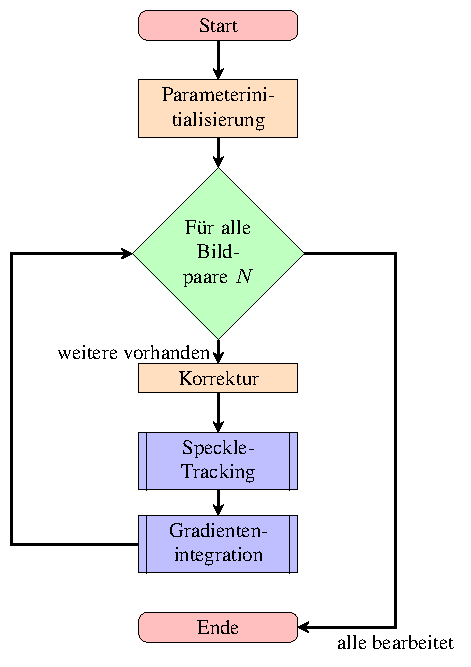
\includegraphics[width=0.4\linewidth]{pdf/graph_main}};
		
		\draw[blue, very thick] (-6.2, -0.0) rectangle (-4.1, -2.6);
		
		\node at (-1,0) {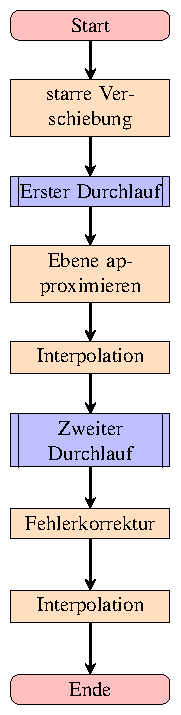
\includegraphics[width=0.16\linewidth]{pdf/graph_speckle}};
		
		\draw[red!50, very thick] (-6, -1.6) rectangle (-4.3, -0.85);
		\draw[red!50, very thick] (-4.3, -0.85) -- (-2, 3.7);
		\draw[red!50, very thick] (-4.3, -1.6) -- (-2, -3.7);
		\draw[red!50, very thick] (-2, -3.7) rectangle (0.1, 3.7);
		
		\draw[blue, very thick] (-1.9, -1.9) rectangle (-0.1, -0.5);
		
		\node[draw=blue] at (2, 0) {MPI};
	\end{tikzpicture}
\end{frame}

\begin{frame}[allowframebreaks, fragile]{Parallele Verarbeitung innerhalb einzelner Bildpaare}
	\textbf{Benennung:} \textit{mpi-advanced}
	\begin{figure}[h]
		\centering
		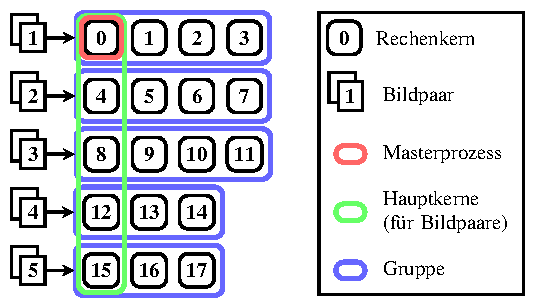
\includegraphics[width=0.5\textwidth]{pdf/parallel}
		\caption[Verteilung]{Verteilung von fünf Bildpaaren auf 18 Rechenknoten}
	\end{figure}
	
	\framebreak
	
	\textbf{Parallelisierung mittels MPI:}
	\begin{lstlisting}[language=Python]
from distributor import Distributor
def initFn():
	global_args = (1, 2)
	local_args = [[1, 5], [2, 6], [3, 7], [4, 8]]
	return (global_args, local_args)
	
def addFn(global_args, local_args):
	(multiply, add) = global_args
	return local_args * multiply + add
	
def mainFn(global_args, local_args, dist):
	return dist.parallel(addFn, global_args, local_args)
	
def exitFn(global_args, result):
	print("The result is", result)
	return 0
	
dist = Distributor(initFn, mainFn, exitFn)
	\end{lstlisting}
	
	\framebreak
	
	\textbf{Parallelisierung mittels joblib:}
	\begin{lstlisting}[language=Python]
from joblib import Parallel, delayed
import multiprocessing

def addFn(array, multiply, add):
	result = []
	for element in array:
		result += [element * multiply + add]
	return result
	
matrix = [[1, 5], [2, 6], [3, 7], [4, 8]]
multiply = 1
add = 2
n_jobs = len(matrix)
result = Parallel()(delayed(addFn)(matrix[k], multiply, add) for k in range(n_jobs))
print("The result is", result)
	\end{lstlisting}
	
	\framebreak
	\textbf{
	Ausgabe}:
	\begin{lstlisting}
The result is [[3, 7], [4, 8], [5, 9], [6, 10]]
	\end{lstlisting}
\end{frame}

\subsection{Optimierung der Performance-Engpässe in Python}
\begin{frame}{Nutzen bereits optimierter Funktionen}
	\centering
	\begin{tikzpicture}
		\node at (-5,0) {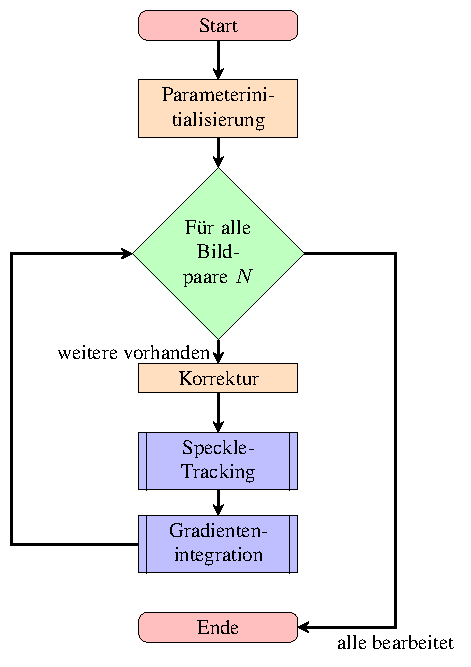
\includegraphics[width=0.4\linewidth]{pdf/graph_main}};
		\node at (-1,0) {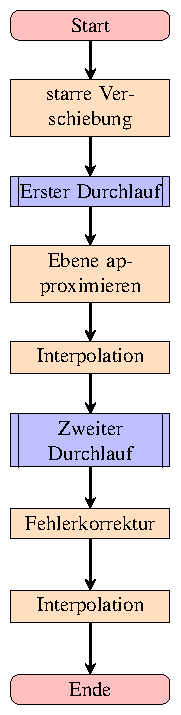
\includegraphics[width=0.16\linewidth]{pdf/graph_speckle}};
		
		\draw[red!50, very thick] (-6, -1.6) rectangle (-4.3, -0.85);
		\draw[red!50, very thick] (-4.3, -0.85) -- (-2, 3.7);
		\draw[red!50, very thick] (-4.3, -1.6) -- (-2, -3.7);
		\draw[red!50, very thick] (-2, -3.7) rectangle (0.1, 3.7);
		
		\draw[blue, very thick] (-1.9, -1.2) rectangle (-0.1, -0.5);
	\end{tikzpicture}
\end{frame}

\begin{frame}[allowframebreaks, fragile]{Nutzen bereits optimierter Funktionen}
	\textbf{Benennung:} \textit{intrinsics}
	
	\textbf{Finden des Maximums einer Matrix:}
	\begin{lstlisting}[language=Python]
for i in range(1, lengthY - 1):
	for j in range(1, lengthX - 1):
		if(nxcorr[i, j] > maxValue):
			maxValue = nxcorr[i, j]
			maxI = i
			maxJ = j
	\end{lstlisting}
	
	\framebreak
	
	\textbf{Finden des Maximums einer Matrix:}
	\begin{lstlisting}[language=Python]
nxcorr_small = nxcorr[1:-1, 1:-1]
(_, maxValue, _, (maxJ, maxI)) = cv2.minMaxLoc(nxcorr_small)
maxI += 1
maxJ += 1
	\end{lstlisting}
	
	\framebreak
	
	\textbf{Berechnung des Signal-Rausch-Verhältnisses:}
	\begin{lstlisting}[language=Python]
avg = 0.0
count = 0
for i in range(lengthY):
	for j in range(lengthX):
		if((i is not maxI) and (j is not maxJ)):
			avg = avg + abs(nxcorr[i,j])
			count = count + 1
			avg = avg / float()count)
			SNr = maxValue / avg
	\end{lstlisting}
\end{frame}

\begin{frame}{Kompilieren - Gesamtes Programm}
	\textbf{Benennung:} \textit{compiled}
	\begin{itemize}
		\item Übersetzen großer Teile des Python-Codes in C mittels Cython
		\item Übersetzen des C-Codes in nativen Bytecode
	\end{itemize}
\end{frame}

\begin{frame}{Kompilieren - Gesamtes Programm}
	\centering
	\begin{tikzpicture}
		\node at (-5,0) {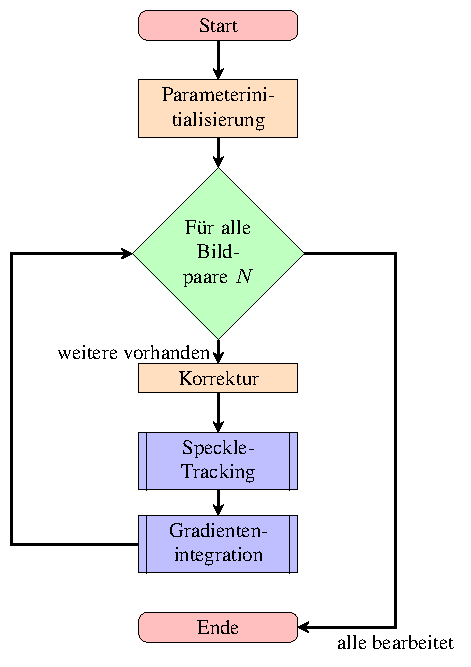
\includegraphics[width=0.4\linewidth]{pdf/graph_main}};
		
		\draw[blue, very thick] (-6.2, -0.0) rectangle (-4.1, -2.6);
	\end{tikzpicture}
\end{frame}

\begin{frame}{Kompilieren - numba}
	\textbf{Benennung:} \textit{numba}
	\begin{itemize}
		\item Annotieren der rechenaufwendigsten Funktionen mittels \texttt{@jit(cached = True)}
		\item just-in-time Übersetzung durch numba beim ersten Aufruf
		\item anschließende Nutzung der Übersetzten Funktionen
	\end{itemize}
\end{frame}


\begin{frame}{Kompilieren - numba}
	\centering
	\begin{tikzpicture}
		\node at (-5,0) {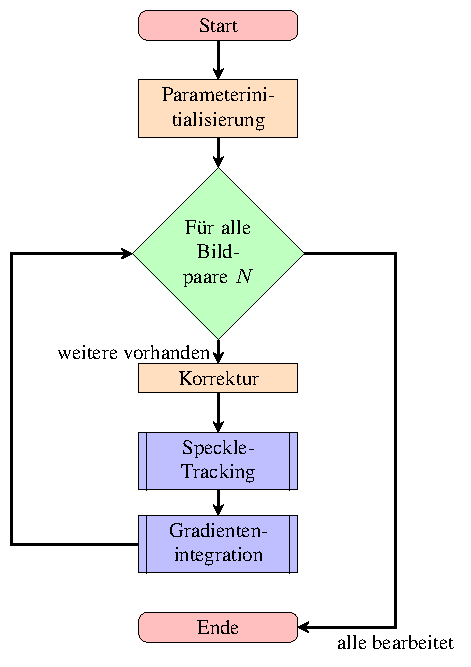
\includegraphics[width=0.4\linewidth]{pdf/graph_main}};
		
		\node at (-1,0) {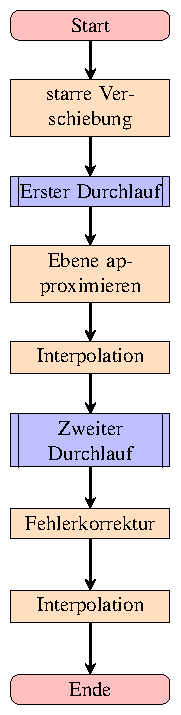
\includegraphics[width=0.16\linewidth]{pdf/graph_speckle}};
		
		\draw[red!50, very thick] (-6, -1.6) rectangle (-4.3, -0.85);
		\draw[red!50, very thick] (-4.3, -0.85) -- (-2, 3.7);
		\draw[red!50, very thick] (-4.3, -1.6) -- (-2, -3.7);
		\draw[red!50, very thick] (-2, -3.7) rectangle (0.1, 3.7);
		
		\draw[blue, very thick] (-1.9, -1.9) rectangle (-0.1, -0.5);
		\draw[blue, very thick] (-1.9, 1.9) rectangle (-0.1, 1.4);
	\end{tikzpicture}
\end{frame}

\begin{frame}{Kompilieren - Cython}
	\textbf{Benennung:} \textit{cython}
	\begin{itemize}
		\item Typisierung der rechenaufwendigsten Funktionen
		\item Übersetzen dieser Funktionen
	\end{itemize}
	
	\vspace{1cm}
	
	\textbf{Benennung:} \textit{compiled-advanced}
	\begin{itemize}
		\item<2> Typisierung der rechenaufwendigsten Funktionen
		\item<2> Übersetzen großer Teile des Python-Codes
	\end{itemize}
\end{frame}

\begin{frame}{Kompilieren - Cython}
	\centering
	\begin{tikzpicture}
		\node at (-5,0) {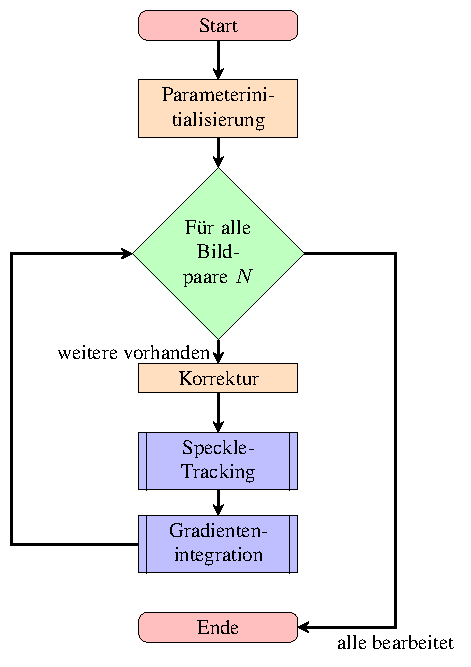
\includegraphics[width=0.4\linewidth]{pdf/graph_main}};
		
		\draw[blue, very thick] (-6.2, -0.0) rectangle (-4.1, -2.6);
		
		\node at (-1,0) {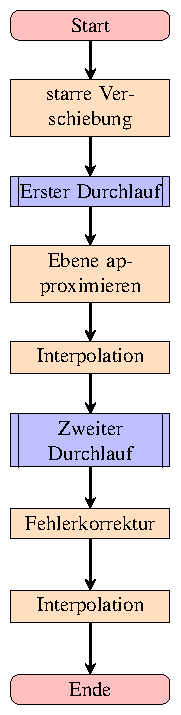
\includegraphics[width=0.16\linewidth]{pdf/graph_speckle}};
		
		\draw[red!50, very thick] (-6, -1.6) rectangle (-4.3, -0.85);
		\draw[red!50, very thick] (-4.3, -0.85) -- (-2, 3.7);
		\draw[red!50, very thick] (-4.3, -1.6) -- (-2, -3.7);
		\draw[red!50, very thick] (-2, -3.7) rectangle (0.1, 3.7);
		
		\draw[green, very thick] (-1.9, -1.9) rectangle (-0.1, -0.5);
		\draw[green, very thick] (-1.9, 1.9) rectangle (-0.1, 1.4);
		
		\node[draw=green] at (2, 0) {typisiert};
		\node[draw=blue] at (2, 1) {zusätzlich übersetzt};
	\end{tikzpicture}
\end{frame}